\chapter{研究背景与挑战}

\section{具身智能与人机共生的发展背景}
人工智能正在由以数字内容处理为主的软件能力，进一步走向能够感知环境、理解任务并作用于物理世界的具身智能。机器人、智能汽车、可穿戴设备、智能家居和新型生产装备持续进入真实场景，使计算不再局限于屏幕之内，而是分布在具有不同形态、位置和功能的物理对象之中。由此，人与机器的关系也开始从“人使用单一工具”转向“人与多类智能体共享环境并协同完成任务”：机器不仅接收预先定义的指令，还会根据环境状态提供信息、提出建议乃至执行动作；人则需要在动态过程中理解机器状态、表达目标并保持必要的监督。

这一变化已成为全球人工智能竞争和产业政策的重要方向。我国《“十四五”机器人产业发展规划》将机器人视为引领产业数字化发展和智能化升级的重要载体，并面向制造、医疗、养老和公共服务等场景推动产品研制与应用拓展\supercite{robot_plan_2021}；2025 年国务院发布《关于深入实施“人工智能+”行动的意见》，进一步提出推动人工智能与经济社会各领域广泛深度融合，加快形成人机协同、跨界融合、共创分享的智能经济和智能社会新形态\supercite{ai_plus_2025}，国家发展改革委随后将人机协作、人机交互和虚实融合概括为智能社会的重要特征，并提出面向人机共生布局新型智能基础设施\supercite{ndrc_symbiosis_2025}。国际上，美国《人工智能行动计划》把自动驾驶、无人机和机器人列为人工智能作用于物理世界的重要形态，提出支持下一代制造并识别机器人制造的供应链挑战\supercite{us_ai_action_plan_2025}；欧盟“Apply AI”战略则把机器人、制造、交通和医疗列为重点领域，通过人工智能工厂、测试验证设施和监管沙盒推动技术由实验室走向市场，同时强调可信、安全和以人为本的应用\supercite{eu_apply_ai_2025}。不同经济体在发展路径和治理方式上各有侧重，但共同表明，人工智能竞争已由模型和算力延伸到智能机器能否进入物理环境、与人协作并形成可持续的生产与服务能力。

政策推动正快速转化为全球产业投入和终端供给。在国内，国家税务总局数据显示，2026 年 1---5 月我国具身智能产业企业销售收入同比增长 22.4\%，机器人本体与整机制造企业销售收入增长 30.1\%，工业企业购进具身智能机器人的金额同比增长 2.3 倍\supercite{china_embodied_tax_2026}；2026 世界机器人大会发布的信息显示，我国人形机器人整机产品已超过 400 款，上半年出货量超过 4 万台，机器人已在多个物流中心参与包裹分拣、在近百家药店承担药品拣选，并开始进入景区讲解、社区巡逻和商业服务等场景\supercite{xinhua_embodied_2026}。在海外，宝马于 2026 年在德国莱比锡工厂启动人形机器人 AEON 的生产试点，使其参与高压电池装配、零部件生产和物料配送；此前美国斯帕坦堡工厂的 Figure 02 已在十个月内参与超过 3 万辆汽车的生产\supercite{bmw_humanoid_2026}。这些中外案例说明，具身智能正由样机展示迁移到真实生产与服务现场，机器也由隔离区域内的固定自动化设备逐步转向能够移动、感知并与工作人员共享作业空间的协作主体。

\begin{figure}[htbp]
  \centering
  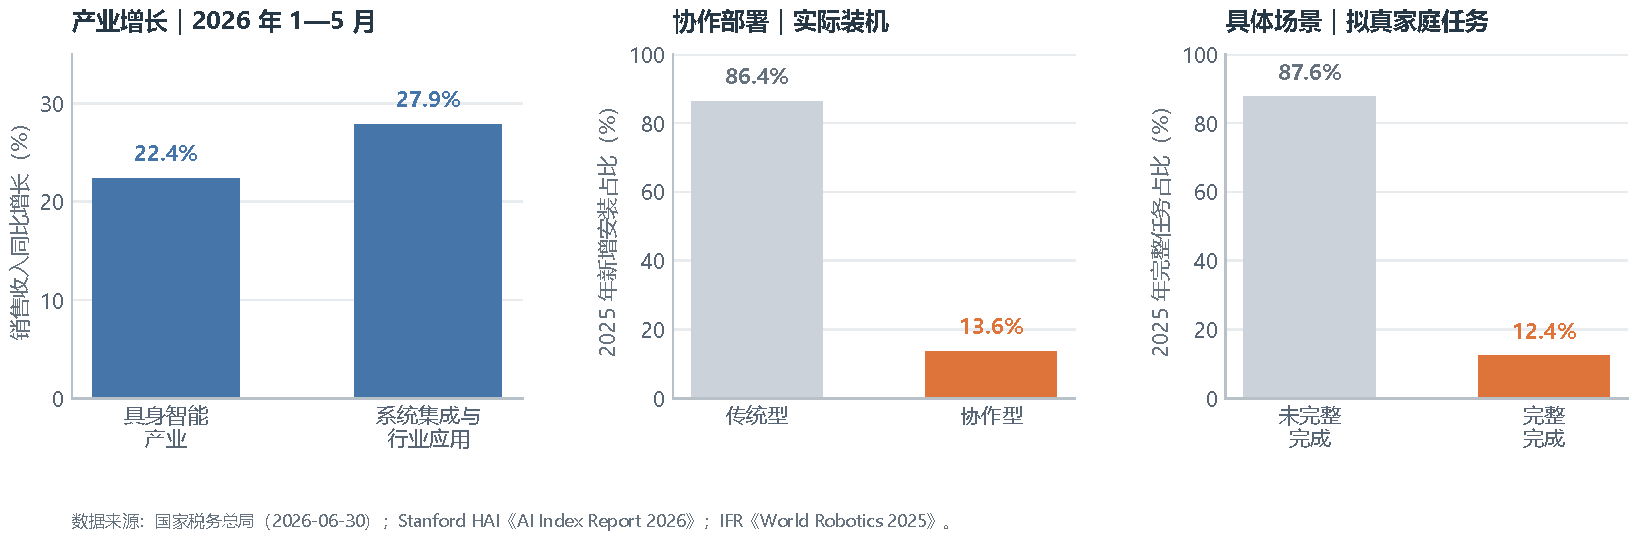
\includegraphics[width=\textwidth]{figs/fig1_1_embodied_ai_landscape.pdf}
  \caption{全球具身智能由政策牵引、产业部署到人机共生挑战的发展态势}
  \label{fig:embodied-ai-development-gap}
\end{figure}

然而，终端数量和展示能力的增长，并不等于人机共生已经成熟。现有案例大多仍集中在物流搬运、部件取放和巡检等边界清晰的任务中，常以少量设备、限定工位或试点项目运行。即使在相对结构化的汽车工厂，宝马仍需先建立统一的数据与接口体系，并在部署过程中增设安全隔离设施、改善厂区 5G 覆盖，再将机器人逐步接入生产流程\supercite{bmw_humanoid_2026}。面向开放环境的行业观察也指出，机器人虽然可以在演示中完成任务，但其速度和可靠性往往尚不足以直接进入工业部署；当不可预测的人进入环境后，机器还必须理解人的语言、手势、姿态和空间指代\supercite{physical_ai_challenge_2026}。

这一现状促使我们思考：\textbf{当具身智能设备已经开始走进工厂、商场、社区和家庭，为什么自然、稳定的人机共生仍未成为普遍现实？} 表面上看，问题表现为机器灵巧性不足、续航有限或模型泛化能力不够；从人机系统的角度看，更深层的原因在于，当前技术主要解决“机器能否完成一个动作”，却尚未充分解决“人如何在复杂现场找到机器、让机器理解自己，并在多个对象之间建立可靠协作关系”。实验室中的一次成功执行通常具有预设目标、已知对象和受控环境，而真实共生场景中的目标、参与者与任务状态会持续变化，两者所需的系统能力并不相同。

首先，现实环境具有开放性和不确定性。物体位置、光照、遮挡和人员活动不断变化，同一指令在不同场景下可能对应不同对象与动作。机器需要把感知结果与物理实体、任务上下文和安全边界联系起来，而不能只复现训练数据中的动作序列。当感知置信度下降或环境发生变化时，系统还要知道何时暂停、请求帮助或把控制权交还给人。这使具身智能的规模化应用不只是模型泛化问题，也是现场状态能否被共同理解的问题。

其次，人机共生环境具有多对象和多主体特征。许多系统仍以“一名用户、一块屏幕、一台预先连接的设备”为基本假设，依靠应用程序、设备名称和菜单层级组织操作。当用户面对多台外观相似的机器人、显示器、传感器或家电时，必须先从网络列表中识别目标，再完成搜索、配对、选择和控制。人在物理空间中已经通过位置、朝向或注视表达了关注对象，数字系统却经常丢失这一信息，导致物理对象、数字身份和交互会话相互分离。

再次，具身智能直接作用于现实世界，交互错误会产生物理后果。系统若选错对象，指令可能被相邻设备执行；若把短暂观察误判为控制意图，又可能触发并非用户所愿的动作。为了规避风险，现有部署常通过隔离区、固定流程和专业人员监督限制机器行为，但这些措施也限制了机器与普通用户自然接触的范围。人机共生因此需要在效率与安全之间取得平衡：既不能让用户为每个简单动作经历冗长配置，也不能把模糊的方向、语音或注视直接解释为高风险命令。

由上述原因可以将人机共生面临的问题归纳为三个系统层面的挑战：一是开放环境下的适应性挑战，机器需要在对象、人员和任务状态持续变化的非结构化现场保持可靠感知与行动，并能在能力边界之外主动求助或交还控制；二是多主体协同挑战，系统需要组织人与多类机器之间的关系，使参与者能够围绕共同目标共享必要的对象、任务和状态信息，而不再依赖“一人一机”的固定配置；三是物理作用下的安全与可信挑战，机器的判断和动作会直接影响现实环境，因而需要控制误操作的后果，并让人能够理解、监督和干预其行为。这三项挑战分别回答机器能否适应现场、多个主体能否形成协作，以及协作能否被安全地接受和使用；其中，如何为人与特定机器建立清晰而低负担的交互关系，是贯穿后两项挑战的基础问题。

综上，具身智能的政策支持、产业投入和终端供给正在全球范围内快速增长，但从可演示、可试点走向可普遍共生，仍存在明显的交互鸿沟。人机共生并不是简单增加机器数量，也不是让机器完全替代人，而是要求人能够自然表达目标，机器能够准确识别对象和意图，双方能够围绕同一任务持续交换状态并处理异常。要跨越这道“最后一公里”，需要从现场空间关系出发重新审视交互入口，使目标发现、身份确认、动作执行与结果反馈围绕同一现实对象连续展开。定向交互由此成为连接具身智能能力与人机共生体验的重要基础。

\section{人机共生环境中的注意力驱动的定向交互}
人机共生环境中的交互具有明确的对象性。用户并不是抽象地向整个环境发出命令，而是在特定时刻希望查看、询问或控制某一个现实对象，例如眼前的机械臂、医疗设备或灯具。当可交互对象由一块屏幕扩展为散布在空间中的大量机器，系统必须先于具体命令回答“用户要与哪一个对象交互”。本文所称的\textbf{定向交互}，即利用用户、交互设备与环境目标之间的空间方向关系，将人的指向映射到特定物理对象，并围绕该对象完成发现、身份确认、命令执行与结果反馈。“定向”既表示人的行为具有空间目标，也要求后续信息仍抵达这个目标，而不是在连接阶段重新退化为对设备列表的搜索。

人的注意力为方向提供了自然线索。人在准备使用物体前，通常会靠近、转头、注视或伸手指向它。不过，心理关注也可以在眼球不转动时发生隐蔽转移，因此注意力并不等同于单一传感器读数，视线只是重要但不完备的观测量\supercite{posner_attention}。本文所称的注意力驱动交互，是指系统利用指向、头向、视线、手部动作和任务上下文估计用户关注的对象，并据此调节目标选择与交互流程；注意力驱动的定向交互则进一步把“用户关注哪里”转化为“系统应与哪一个现实对象建立交互”。其目的不是用眼睛替代鼠标，而是利用人已经自然表达的空间关注，减少重复搜索、命名和配对。

定向交互的发展始于对自然指代行为的数字化。1980 年，麻省理工学院的 ``Put-That-There'' 系统将手势指向与语音结合，由方向回答“哪个对象和位置”，由语音表达动作\supercite{bolt_put_that_there}。1990 年，Jacob 将眼动用于界面目标选择，同时指出眼睛既承担观察任务，又可能被解释为控制命令，从而产生“米达斯接触”问题\supercite{jacobgaze}。进入普适计算阶段，研究重点由操作一台计算机转向管理多设备环境中的注意力。卡内基梅隆大学 2002 年提出 Project Aura，将人的注意力视为普适计算中最稀缺的资源，通过感知用户任务与可用设备减少配置和迁移造成的打断\supercite{project_aura}；随后形成的注意用户界面主张系统根据自己处于注意力前景还是背景决定何时响应\supercite{attentive_user_interfaces}。EyePliances 给出了现实家电实例：电视在无人观看时暂停，AuraLamp 只有在用户看向它时才接受语音命令\supercite{eyepliances}。这些工作确立了“以方向确定目标、以其他线索确认操作”的基本范式。

移动计算、增强现实和可穿戴感知进一步把这一范式带入三维空间。ubiGaze 利用头戴眼动设备把凝视手势附着到真实物体\supercite{ubigaze}，Gaze+Pinch 则以凝视指定目标、以捏合手势确认和操纵，形成“眼睛选择、手部承诺”的多模态分工\supercite{gaze_pinch}。面向物联网，Snap-To-It、Scenariot 和 BLEselect 分别探索借助目标图像、增强现实空间映射和蓝牙到达角选择现实设备\supercite{snaptoit,scenariot,bleselect}。目前研究又开始把眼动、手势、场景视觉和历史行为结合，用注意力帮助情境智能体理解用户任务。2025 年的研究表明，将此前的物体注视轨迹加入视觉语言模型上下文，可以改善模型对当前关注对象和下一步交互对象的判断\supercite{gaze_contextual_ai}。研究重心由瞬时“看向哪里”逐步扩展到持续的对象关联与任务情境。

注意力驱动交互也已进入商业空间计算平台。HoloLens 2 支持头部凝视、眼动凝视和凝视停留，适用于维修人员双手被工具占用且现场噪声不利于语音控制的场景\supercite{hololens_gaze_dwell}；Apple Vision Pro 则把“看向对象并捏合手指”作为 visionOS 的主要间接交互方式\supercite{visionos_interaction}。这些系统证明了注意力方向可以减少光标移动和远距离伸手，但其成熟体验主要建立在平台已知的窗口、三维模型和空间锚点之上。对于未预先建模的机械臂、家电或公共设施，系统仍需完成物体识别、数字身份关联和通信授权，才能把一次“看向”转化为现实操作。
我们不禁思考：\textbf{当设备已经能够测量用户的指向、头向和视线，为什么注意力驱动定向交互仍未成为普遍能力？} 例如，在装有两台同型号机械臂的车间中，眼镜可能测得用户正看向左侧机械臂，相机也识别出“机械臂”类别，但无线网络只返回两个相似的设备名称。系统仍不知道左侧实体对应哪个网络地址，也无法保证启动命令不会发给另一台机器。问题的关键因此不是能否获得一个方向，而是该方向能否被可靠地转化为正确对象、真实意图和一致的信息通道。

由方向线索确定注意目标仍存在较大不确定性。手持设备指向较明确，却要求用户举起并对准；头向便于持续获取，却只能粗略表示视野中心；眼动最接近视觉注意，但会受到标定误差、个体差异、设备滑移和自然扫视影响。日常条件下眼动的准确度和精密度会随用户、目标位置与设备状态明显变化\supercite{everydaygaze}；在三维场景中，角度误差还会随距离放大，同一视线附近可能存在相邻、同类或不同深度的多个物体。将测得的 gaze point 映射为具有语义的 gaze object，本身仍是尚未完全解决的问题\supercite{gaze_to_object_mapping}。此外，用户查看灯具可能只是观察环境，并不意味着希望开灯；人在寻找零件或巡视设备时也会自然扫过大量对象。因此，目标解析不仅要融合指向、头向和视线以判断“关注什么”，还要结合动作与上下文判断当前关注是否足以启动交互。

确定物理目标后，系统仍需将其与唯一的数字身份对齐。相机感知和 Wi-Fi、蓝牙发现分别回答“看见了什么”和“附近有什么设备”，却不能证明视野中的某个实体就是设备列表中的某个地址。在同型号设备密集部署、对象移动或遮挡的场景中，依据外观类别、设备名称或邻近关系建立映射都容易产生歧义。二维码、预注册数据库和空间锚点可以辅助关联，但会引入扫描、部署与维护开销，并可能随设备位置或环境布局变化而失效。物理对象与数字身份之间的断裂，使正确的空间选择仍可能转化为错误的网络连接。

建立连接也不意味着交互已经完成。若每次注视都触发命令，会产生严重误操作；若一律要求长时间停留、语音或手势确认，又会抵消注意力交互的效率。Gaze+Pinch 通过“凝视选择、手势确认”缓解米达斯接触，但眼手配合、目标切换和持续操纵仍缺乏统一规则\supercite{gaze_pinch_challenges}。当用户移动、视线离开或链路短时中断时，系统还需要判断应保持会话、重新验证还是切换目标，并将执行状态和结果返回给用户，否则一次正确选择仍难形成可控的交互过程。

据此，注意力驱动定向交互可归纳为三项相互衔接的核心挑战：\textbf{一是注意目标解析挑战}，需要从带有噪声的多模态方向线索中确定用户关注的现实对象，并判断其是否进入交互状态；\textbf{二是物理--数字身份对齐挑战}，需要把选中的现实实体可靠映射到唯一的设备身份和网络地址；\textbf{三是交互闭环保持挑战}，需要根据操作风险设置确认机制，并在移动、遮挡和目标切换过程中维持命令、状态与反馈的一致性。三者依次回答“面向谁”“连接谁”和“如何持续交互”，共同将人的空间注意转化为可执行、可验证的现实操作。

综上，注意力驱动的定向交互已经由屏幕指向和凝视输入，发展到多设备注意力管理、空间计算与情境智能，但现有成果仍未完全贯通现实对象感知、身份确认和数据传输。要使“所指”“所看”可靠地转化为“所交互”，一方面需要\textbf{定向感知技术}提取注意方向并定位目标，另一方面需要\textbf{定向通信技术}利用空间约束核验目标身份、建立局部链路并返回反馈。光学技术同时具备成像感知、视距传播与波束空间约束能力，为统一注意方向、物理对象和信息通道提供了自然基础。

\section{面向定向交互的通信感知技术发展}
上一节指出，注意力驱动定向交互需要把人的注意方向绑定到物理对象，再将其转化为安全、连续的数字连接，即同时回答“目标在哪里”和“目标是谁”。视觉感知能够恢复对象的位置、类别和姿态，射频通信能够发现节点并维持连接，但二者的空间对象与网络身份并不天然对应。光学信号既可成像又可传输数据，并受光束方向、接收视场和遮挡关系约束，因此为统一注意方向、现实对象与信息通道提供了自然基础。

从实现机制看，光学通信通常采用强度调制与直接检测：发光器件以人眼难以察觉的速度改变光强，光电二极管或相机将接收光转换为电信号并恢复数据。发射光束越窄、接收视场越小，链路覆盖的空间范围越集中，不同方向上的对象也越容易分离。因此，光学用于定向交互的价值不仅在于频谱和速率，更在于通过物理传播范围缩小候选集合，使信息来源与用户面对的空间方向建立直接联系。

光学技术首先被用于\textbf{对象感知与空间锚定}。相机通过外观、二维码或人工标记识别目标，1999 年的 ARToolKit 推动了视觉标记在增强现实注册中的应用\supercite{artoolkit_1999}；2002 年的 FindIT 则使用手持光束唤醒匹配标签，使“照向哪里”直接决定“查询谁”\supercite{findit}。InfoLED、LightAnchors 等系统进一步利用设备指示灯或场景点光源，将数字信息锚定到现实位置\supercite{infoled,lightanchors}。这一路线建立了空间选择能力，但静态标记只能提供预存信息，识别结果仍需借助额外映射才能转化为控制链路。

高效 LED 与光电器件的普及推动技术由对象识别走向\textbf{双向光学通信}。2011 年，IEEE 802.15.7 定义了短距离可见光通信机制，LiFi 随后将单条光链路扩展为支持多用户接入和移动切换的无线网络\supercite{ieee_802_15_7,what_is_lifi}。产业界也开始推动落地：Signify 于 2019 年推出 Trulifi 商用系统，2023 年发布的 IEEE 802.11bb 则将光通信纳入无线局域网标准体系\supercite{signify_trulifi,ieee_802_11bb}。这些里程碑表明，光已由单向信息载体发展为可与现有网络协同的接入媒介。

然而，大量现实对象若采用主动光发射器回传，会带来持续供电、方向对准和硬件成本问题。由此形成的\textbf{无源光学回传}路线，使用主动读写器照射目标，以逆反射材料将入射光送回光源附近，并通过液晶等低功耗调制器在回波上编码身份与状态。Retro-VLC、PassiveVLC 和 TurboBoost 等工作逐步验证并提升了这类双向链路的距离、速率与环境适应性\supercite{retrovlc,passivevlc,turboboost}。当手机或眼镜指向目标时，窄光束先筛选候选对象，近原路返回的信号再确认其身份，使“指向哪个物体”与“数据来自哪个设备”在同一现场链路中得到验证，交互入口也由手持指向逐步走向头向和视线驱动。

方向性既是光学的优势，也是其限制。窄光束和小接收视场能够缩小候选范围、降低误绑定，却容易受到环境光、入射角、人体遮挡和用户移动影响，不适合独立承担长时间连接。射频链路则覆盖广、非视距能力强且基础设施成熟，但难以判断用户关注的是哪个现实对象。这种互补性推动技术路线走向\textbf{光学与射频混合}：定向光链路负责发现目标并读取身份、能力或临时凭据，Wi-Fi、蓝牙等射频网络随后承载可穿越短时遮挡的持续会话。已有 LiFi 与 Wi-Fi 混合网络也验证了局部光接入与广域无线覆盖的协同价值\supercite{hybrid_lifi_wifi}。

相较于单一媒介，混合路线可以在建立射频连接前利用空间方向缩小候选范围，并在选择完成后容忍转头、移动与暂时遮挡；同时，低功耗光标签只需交换身份、授权和少量状态，大数据传输与长期控制可以复用成熟射频设施。其关键不在于简单并列两条链路，而在于保证光学身份与射频地址一致，并合理设计遮挡后的保持、重新验证和目标切换机制，从而将第 1.2 节提出的注意目标解析、物理--数字身份对齐和交互闭环保持落实为完整交互流程。

基于上述脉络，本文以光学通信感知一体化作为注意方向与现实对象之间的入口，并探索光学与射频协同：首先利用手机指向和可见光逆反射实现对象选择与信息回传，继而将入口迁移到智能眼镜和近红外双向链路，进一步结合眼动追踪、可调光束与多模态意图判别，并在目标验证后转入可持续的无线会话，使交互由“所指”走向“所看”与“所欲”。
